\documentclass{minimal}
\usepackage{graphicx,color}
\usepackage[papersize={576.00bp,432.00bp},text={576.00bp,432.00bp}]{geometry}
\begin{document}
\centering
% Title: glps_renderer figure
% Creator: GL2PS 1.3.8, (C) 1999-2012 C. Geuzaine
% For: Octave
% CreationDate: Sat Nov 11 01:42:34 2017
\setlength{\unitlength}{1pt}
\begin{picture}(0,0)
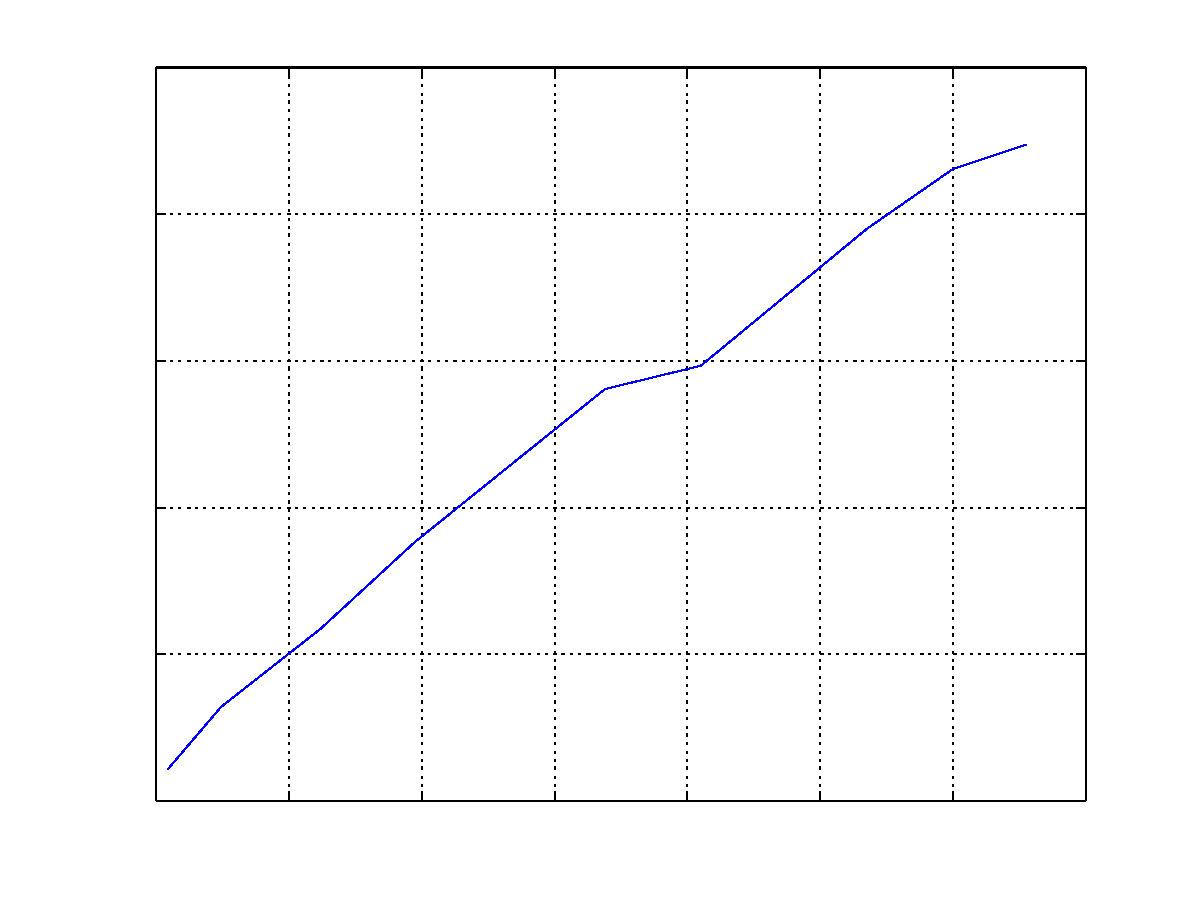
\includegraphics{temp-inc}
\end{picture}%
\begin{picture}(576,432)(0,0)
\fontsize{16}{0}
\selectfont\put(74.88,42.5189){\makebox(0,0)[t]{\textcolor[rgb]{0,0,0}{{0}}}}
\fontsize{16}{0}
\selectfont\put(138.651,42.5189){\makebox(0,0)[t]{\textcolor[rgb]{0,0,0}{{1}}}}
\fontsize{16}{0}
\selectfont\put(202.423,42.5189){\makebox(0,0)[t]{\textcolor[rgb]{0,0,0}{{2}}}}
\fontsize{16}{0}
\selectfont\put(266.194,42.5189){\makebox(0,0)[t]{\textcolor[rgb]{0,0,0}{{3}}}}
\fontsize{16}{0}
\selectfont\put(329.966,42.5189){\makebox(0,0)[t]{\textcolor[rgb]{0,0,0}{{4}}}}
\fontsize{16}{0}
\selectfont\put(393.737,42.5189){\makebox(0,0)[t]{\textcolor[rgb]{0,0,0}{{5}}}}
\fontsize{16}{0}
\selectfont\put(457.509,42.5189){\makebox(0,0)[t]{\textcolor[rgb]{0,0,0}{{6}}}}
\fontsize{16}{0}
\selectfont\put(521.28,42.5189){\makebox(0,0)[t]{\textcolor[rgb]{0,0,0}{{7}}}}
\fontsize{16}{0}
\selectfont\put(69.8755,47.52){\makebox(0,0)[r]{\textcolor[rgb]{0,0,0}{{0}}}}
\fontsize{16}{0}
\selectfont\put(69.8755,117.936){\makebox(0,0)[r]{\textcolor[rgb]{0,0,0}{{10}}}}
\fontsize{16}{0}
\selectfont\put(69.8755,188.352){\makebox(0,0)[r]{\textcolor[rgb]{0,0,0}{{20}}}}
\fontsize{16}{0}
\selectfont\put(69.8755,258.768){\makebox(0,0)[r]{\textcolor[rgb]{0,0,0}{{30}}}}
\fontsize{16}{0}
\selectfont\put(69.8755,329.184){\makebox(0,0)[r]{\textcolor[rgb]{0,0,0}{{40}}}}
\fontsize{16}{0}
\selectfont\put(69.8755,399.6){\makebox(0,0)[r]{\textcolor[rgb]{0,0,0}{{50}}}}
\fontsize{16}{0}
\selectfont\put(298.08,23.5189){\makebox(0,0)[t]{\textcolor[rgb]{0,0,0}{{Current (A)}}}}
\fontsize{16}{0}
\selectfont\put(45.8755,223.56){\rotatebox{90}{\makebox(0,0)[b]{\textcolor[rgb]{0,0,0}{{Temperature rise ($^oC$)}}}}}
\fontsize{12}{0}
\selectfont\put(106.766,350.309){\makebox(0,0)[l]{\textcolor[rgb]{0,0,0}{{F(x) = 6.56761x+3.46169}}}}
\fontsize{12}{0}
\selectfont\put(106.766,315.101){\makebox(0,0)[l]{\textcolor[rgb]{0,0,0}{{$R^2$ = 0.992566}}}}
\end{picture}
\end{document}
